\section{Matrix Based CFPQ for Single-Path Semantics}
In this section, we propose the matrix-based algorithm for CFPQ w.r.t. the single-path query semantics (see listing~\ref{lst:algo2}). This algorithm constructs the set of matrices $T$ with PathIndexes as elements.
{\small
	\begin{algorithm}
		\floatname{algorithm}{Listing}
		\begin{algorithmic}[1]
			\caption{CFPQ algorithm w.r.t. single-path query semantics}
			\label{lst:algo2}
			\Function{evalCFPQ}{$D=(V,E), G=(N,\Sigma,P)$}
			\State{$n \gets$ |V|}
			\State{$T \gets \{T^{A_i} \mid A_i \in N, T^{A_i}$ is a matrix $n \times n$, $T^{A_i}_{k,l} \gets \bot$ \} }
			\ForAll{$(i,x,j) \in E$, $A_k \mid A_k \to x \in P$}
			%\Comment{Matrices initialization}
			%\For{$A_k \mid A_k \to x \in P$}
			{$T^{A_k}_{i,j} \gets (i,j,i,1,1)$}
			%\EndFor
			\EndFor
			\For{$A_k \mid A_k \to \varepsilon \in P$}
			{$T^{A_k}_{i,i} \gets (i,i,i,1,0)$}
			\EndFor
			
			\While{any matrix in $T$ is changing}
			%\Comment{Transitive closure calculation}
			\For{$A_i \to A_j A_k \in P$}
			{ $T^{A_i} \gets T^{A_i} + (T^{A_j} \odot T^{A_k})$ } 
			\EndFor
			\EndWhile
			\State \Return $T$
			\EndFunction
		\end{algorithmic}
	\end{algorithm}
}

After constructing the set of matrices $T$ for every node pair $i, j$ and nonterminal $A$ we can extract a path $i \pi j$ from $i$ to $j$ such that $A \xRightarrow[G]{*} l(\pi)$ if such path exists. We also propose the algorithm (see listing~\ref{lst:algo3}) for extracting one of those paths which forms a string with minimal height of derivation tree. Our algorithm returns the empty path $[]$ only if $i = j$ and $A \to \varepsilon \in P$. Note that if the PathIndex for given $i,j,A$ is equal to $\bot$ then our algorithm returns a special path $\pi_{\emptyset}$ to denote that such a path does not exist.

{\small
	\begin{algorithm}
		\floatname{algorithm}{Listing}
		\begin{algorithmic}[1]
			\caption{Path extraction algorithm}
			\label{lst:algo3}
			\Function{extractPath}{$i, j, A, T=\{T^{A_i}\}, G=(N,\Sigma,P)$}
			\State{$index \gets T^{A}_{i,j}$ }
			
			\If{$index = \bot$}
			\State \Return $\pi_{\emptyset}$
			\Comment{Such a path does not exist}
			\EndIf
			
			\If{$index.height = 1$}
			\If{$index.length = 0$}
			\State \Return $[]$
			\Comment{Return an empty path}
			\EndIf
			\ForAll{$ x \mid (i,x,j) \in E$}
			\If{$A \to x \in P$}
			\State \Return $[(i,x,j)]$
			\Comment{Return a path of length one}
			\EndIf
			\EndFor
			\EndIf
			
			\ForAll{$A \to B C \in P$}
			\State{$index_B \gets T^{B}_{i,index.middle}$ }
			\State{$index_C \gets T^{C}_{index.middle,j}$ }			
			\If{$(index_B \neq \bot) \wedge (index_C \neq \bot)$}
			\State{$maxH \gets max(index_B.height, index_C.height)$ }
			\If{$index.height = maxH + 1$}
			
						
			\State{$\pi_1 \gets$ \Call{extractPath}{$i, index.middle, B, T, G$}}
			\State{$\pi_2 \gets$ \Call{extractPath}{$index.middle, j, C, T, G$}}
			\State \Return $\pi_1 + \pi_2$
			\EndIf
			\EndIf
			\EndFor
			\EndFunction
		\end{algorithmic}
	\end{algorithm}
}

\subsection{Correctness}

Let $T^{(p)} = \{T^{(p), A_i}\}$ be a constructed matrix $T$ by the algorithm in listing~\ref{lst:algo2} after $p-1$ loop iterations for $p \geq 2$, and $T^{(1)} = \{T^{(1), A_i}\}$ be a constructed matrix $T$ by this algorithm after initialization in lines 3-5. Note that the matrix $T$ returned by this algorithm is equal to $\sum_{p = 1}^{\infty} T^{(p)}$. Then the following lemma and theorem hold.

\begin{lemma}\label{lemma:correctness}
	Let $D = (V,E)$ be a graph, let $G =(N,\Sigma,P)$ be a grammar. Then for any $i, j$ and for any non-terminal $A \in N$, $index = T^{(p),A}_{i,j}$ and $index = (i,j,k,h,l) \neq \bot$ iff $(i,j) \in R_A$ and $i \pi j$, such that there is a derivation tree of the minimal height $h \leq p$ for the string $l(\pi)$  of length $l$ and a context-free grammar $G_A = (N,\Sigma,P,A)$.
\end{lemma}
\begin{proof}(Proof by Induction)
	
	\textbf{Base case}: Show that the lemma holds for $p = 1$. For any $i, j$ and for any non-terminal $A \in N$, $(i,j,k,h,l) = T^{(1), A}_{i,j}$ iff there is either $i \pi j$ of length $1$ that consists of a unique edge $e$ from the node $i$ to the node $j$ and $(A \rightarrow x) \in P$, where $x = l(\pi)$, or $i = j$ and $(A \rightarrow \varepsilon) \in P$, where $\varepsilon = l(\pi)$. Therefore $(i,j) \in R_A$ and there is a derivation tree of the minimal height $h = p = 1$, shown on Figure~\ref{tree1}, for the string $x$ and a context-free grammar $G_A = (N,\Sigma,P,A)$. Thus, it has been shown that the lemma holds for $p = 1$.
	
	\begin{figure}[h!]
		\centering
		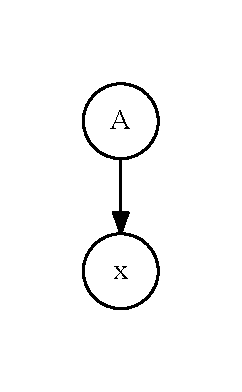
\includegraphics[width=2cm]{pictures/tree1.pdf}
		\caption{The derivation tree of the minimal height $p = 1$ for the string $x = l(\pi)$ where $x \in \Sigma \cup \{\varepsilon\}$.}
		\label{tree1}
	\end{figure}
	
	\textbf{Inductive step}: Assume that the lemma holds for any $p \leq (q - 1)$ and show that it also holds for $p = q$, where $q \geq 2$.
	
	The index $(i,j,k,h,l) = T^{(q),A}_{i,j}$ iff there is exists a rule $(A \to B C) \in P$ such that $(i,j,k,h,l) = M_{i,j}$ where $M = T^{(q-1),A} + (T^{(q-1),B} \odot T^{(q-1),C})$. 
	
	Let $(i,j,k,h,l) = T^{(q-1),A}_{i,j}$. By the inductive hypothesis, $(i,j,k,h,l) = T^{(q-1),A}_{i,j}$ iff $(i,j) \in R_A$ and there exists $i \pi j$, such that there is a derivation tree of the minimal height $h \leq (q-1)$ for the string $l(\pi)$ and a context-free grammar $G_A = (N,\Sigma,P,A)$. The statement of the lemma holds for $p = q$ since the height $h$ of this tree is also less than or equal to $q$.
	
	Now, let $(i,j,k,h,l) = (T^{(q-1),B} \odot T^{(q-1),C})_{i,j}$. By the definition of the binary operation $\odot$, $(i,j,k,h,l) = (T^{(q-1),B} \odot T^{(q-1),C})_{i,j}$ iff there are $r=k$, $(i,r,\_,h_1,l_1) = T^{(q-1),B}_{i,r}$ and $(r,j,\_,h_2,l_2) = T^{(q-1),C}_{r,j}$, such that $q = max(h_1, h_2) + 1$, $l = l_1 + l_2$. Hence, by the inductive hypothesis, there are $i \pi_1 r$ and $r \pi_2 j$, such that $(i,r) \in R_B$ and $(r,j) \in R_C$, and there are the derivation trees $T_B$ and $T_C$ of minimal heights $h_1 \leq (q-1)$ and $h_2 \leq (p-1)$ for the strings $w_1 = l(\pi_1)$, $w_2 = l(\pi_2)$ and the context-free grammars $G_B$, $G_C$ respectively. Thus, the concatenation of paths $\pi_1$ and $\pi_2$ is $i \pi j$, where $(i,j) \in R_A$ and there is a derivation tree of the minimal height $h = 1 + max(h_1, h_2)$, shown on Figure~\ref{tree2}, for the string $w = l(\pi)$ of length $l = l_1 + l_2$ and a context-free grammar $G_A$.
	\begin{figure}[h!]
		\centering
		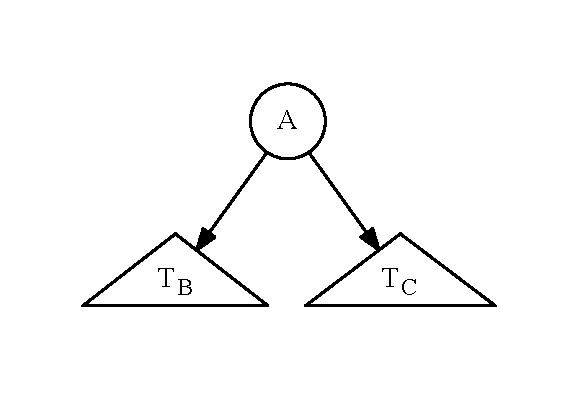
\includegraphics[width=5cm]{pictures/tree2.pdf}
		\caption{The derivation tree of the minimal height $h = 1 + max(h_1, h_2)$ for the string $w = l(\pi)$, where $T_B$ and $T_C$ are the derivation trees for strings $w_1$ and $w_2$ respectively.}
		\label{tree2}
	\end{figure}
	
	The statement of the lemma holds for $p = q$ since the minimal height $h = 1 + max(h_1, h_2) \leq q$. This completes the proof of the lemma.
\end{proof}

\begin{mytheorem}\label{thm:correct}
	Let $D = (V,E)$ be a graph and let $G =(N,\Sigma,P)$ be a grammar. Then for any $i, j$ and for any non-terminal $A \in N$, $index = T^A_{i,j}$ and $index = (i,j,k,h,l) \neq \bot$ iff $(i,j) \in R_A$ and $i \pi j$, such that there is a derivation tree of the minimal height $h$ for the string $l(\pi)$ of length $l$ and a context-free grammar $G_A = (N,\Sigma,P,A)$.
\end{mytheorem}
\begin{proof}
	
	Since the matrix $T = \sum_{p = 1}^{\infty} T^{(p)}$ for any $i, j$ and for any non-terminal $A \in N$, $index = T^A_{i,j}$ and $index = (i,j,k,h,l) \neq \bot$ iff there is $p \geq 1$, such that $index \in T^{(p),A}_{i,j}$. By the lemma~\ref{lemma:correctness}, $index = T^{(p),A}_{i,j}$ iff $(i,j) \in R_A$ and $i \pi j$, such that there is a derivation tree of the minimal height $h \leq p$ for the string $l(\pi)$  of length $l$ and a context-free grammar $G_A = (N,\Sigma,P,A)$. This completes the proof of the theorem.
\end{proof}

Now, using the theorem~\ref{thm:correct} and induction on the length of the path, it can be easily shown that the following theorem holds.

\begin{mytheorem}\label{thm:correct_extraction}
	Let $D = (V,E)$ be a graph, let $G =(N,\Sigma,P)$ be a grammar and $T$ be a set of matrices returned by the algorithm in listing~\ref{lst:algo2}. Then for any $i, j$ and for any non-terminal $A \in N$ such that $index = T^A_{i,j}$ and $index = (i,j,k,h,l) \neq \bot$, the algorithm in listing~\ref{lst:algo3} for these parameters will return a path $i \pi j$ such that $(i,j) \in R_A$ and there is a derivation tree of the minimal height $h$ for the string $l(\pi)$ of length $l$ and a context-free grammar $G_A = (N,\Sigma,P,A)$.
\end{mytheorem}

We can, therefore, determine whether $(i,j) \in R_A$ by asking whether $T^A_{i,j} = \bot$. Also, we can extract such a path which forms a string with a derivation tree of minimal height by using our algorithm in listing~\ref{lst:algo3}. Thus, we show how the context-free path query evaluation w.r.t. the single-path semantics can be solved in terms of matrix operations.

\subsection{Complexity}

Denote the number of elementary operations executed by the algorithm of multiplying two $n \times n$ matrices with PathIndexes as $MM(n)$. Also, denote the number of elementary operations, executed by the matrix element-wise + operation of two $n \times n$ matrices with PathIndexes as $MA(n)$. Since the line \textbf{7} of the algorithm in listing~\ref{lst:algo2} is executed no more than $|V|^2|N|$ times, the following theorem holds.

\begin{mytheorem}\label{thm:time}
	Let $D = (V,E)$ be a graph and let $G =(N,\Sigma,P)$ be a grammar. The algorithm in listing~\ref{lst:algo2} calculates the set of matrices $T$ in $O(|V|^2|N|^3(MM(|V|) + MA(|V|)))$.
\end{mytheorem}

Also, denote the time complexity of the access to the PathIndex in the $n \times n$ matrix as $Access(n)$. Then the following theorem on the time complexity of the path extraction algorithm holds.

\begin{mytheorem}\label{thm:time_extraction}
	Let $D = (V,E)$ be a graph, let $G =(N,\Sigma,P)$ be a grammar and $T$ be a set of matrices returned by the algorithm in listing~\ref{lst:algo2}. Then for any $i, j$ and for any non-terminal $A \in N$ such that $index = T^A_{i,j}$ and $index = (i,j,k,h,l) \neq \bot$, the algorithm in listing~\ref{lst:algo3} for these parameters calculates a path $i \pi j$ in $O(l \times N \times Access(|V|))$.
\end{mytheorem}

\subsection{An Example}
In this section, we provide a step-by-step demonstration of the proposed algorithms. For this, we consider the example with the worst-case time complexity.

The \textbf{example query} is based on the context-free grammar $G = (N, \Sigma, P)$ of the worst-case example query where:
\begin{itemize}
	\item the set of non-terminals $N = \{S\}$;
	\item the set of terminals $\Sigma = \{a, b\}$;
	\item the set of production rules $P$ is presented on Figure~\ref{ProductionRulesWorsCaseExample}.
\end{itemize}

\begin{figure}[h]
	\[
	\begin{array}{rccl}
	0: & S & \rightarrow & \text{\emph{a}} \ S \ \text{\emph{b}} \\
	1: & S & \rightarrow & \text{\emph{a}} \ \text{\emph{b}} \\ 
	\end{array}
	\]
	\caption{Production rules for the worst-case example.}
	\label{ProductionRulesWorsCaseExample}
\end{figure}

Since the proposed algorithm processes only grammars in Chomsky normal form, we first transform the grammar $G$ into an equivalent grammar $G' = (N', \Sigma', P')$ in normal form, where:
\begin{itemize}
	\item the set of non-terminals $N' = \{S, S_1, A, B\}$;
	\item the set of terminals $\Sigma' = \{a, b\}$;
	\item the set of production rules $P'$ is presented on Figure~\ref{ProductionRulesExampleQueryCNF}.
\end{itemize}

\begin{figure}[h]
	\[
	\begin{array}{rccl}
	0: & S & \rightarrow & A \ B \\
	1: & S & \rightarrow & A \ S_1 \\
	2: & S_1 & \rightarrow & S \ B \\
	3: & A & \rightarrow & \text{\emph{a}} \\ 
	4: & B & \rightarrow & \text{\emph{b}} \\ 
	\end{array}
	\]
	\caption{Production rules for the example query grammar in normal form.}
	\label{ProductionRulesExampleQueryCNF}
\end{figure}

We run the query on a graph, presented on Figure~\ref{Example_Graph}. We provide a step-by-step demonstration of the work with the given graph $D$ and grammar $G'$ of the algorithm in listing~\ref{lst:algo2}. After the matrix initialization in lines \textbf{3-5} of this algorithm, we have a matrix $T^{(1)}$, presented on Figure~\ref{ExampleQueryInitMatrix}.

\begin{figure}[h]
	\[
	T^{(1),A} = \begin{pmatrix}
	\bot & (0,1,0,1,1)       & \bot & \bot       \\
	\bot & \bot & (1,2,1,1,1)       & \bot \\
	(2,0,2,1,1)       & \bot & \bot & \bot \\
	\bot       & \bot & \bot & \bot \\
	\end{pmatrix}
	\]
	\[
	T^{(1),B} = \begin{pmatrix}
	\bot & \{A\}       & \bot & (0,3,0,1,1)       \\
	\bot & \bot & \{A\}       & \bot \\
	\{A\}       & \bot & \bot & \bot \\
	(3,0,3,1,1)      & \bot & \bot & \bot \\
	\end{pmatrix}
	\]
	\caption{The initial matrix for the example query. The PathIndexes $T^{(1),S_1}_{i,j}$ and $T^{(1),S}_{i,j}$ are equal to $\bot$ for every $i,j$.}
	\label{ExampleQueryInitMatrix}
\end{figure}

After the initialization the only matrices which will be updated are $T^{S_1}$ and $T^{S}$. These matrices obtained after first loop iteration is shown on Figure~\ref{ExampleQueryFirstIteration}.

\begin{figure}[h]
	\[
	T^{(2),S} = \begin{pmatrix}
	\bot & \bot       & \bot & \bot       \\
	\bot & \bot & \bot       & \bot \\
	\bot       & \bot & \bot & (2,3,0,2,2) \\
	\bot       & \bot & \bot & \bot \\
	\end{pmatrix}
	\]
	\caption{The first iteration of computing the transitive closure for the example query. The PathIndexes $T^{(1),S_1}_{i,j}$ are equal to $\bot$ for every $i,j$.}
	\label{ExampleQueryFirstIteration}
\end{figure}

When the algorithm at some iteration finds new paths for some nontermial in the graph $D$, then it adds corresponding PathIndexes to the matrix for this nonterminal. For example, after the first loop iteration, PathIndex $(2,3,0,2,2)$ is added to the matrix $T^{S}$. This PathIndex is added to the element with a row index $i = 2$ and a column index $j = 3$. This means, that there is $i\pi j$ (a path $\pi$ from the node 2 to the node 3), such that $S \xRightarrow[G]{*} l(\pi)$, this path obtained by concatenation of smaller paths via node 0, the length of path is equal to 2, and the derivation tree for the string $l(pi)$ has a height 2.

The calculation of the transitive closure is completed after $k$ iterations, when a fixpoint is reached: $T^{(k)} = T^{(k+1)}$. For the example query, $k = 13$ since $T_{13} = T_{14}$. The resulted matrices are presented on Figure~\ref{ExampleQueryFinalMatrices}.

\begin{figure}[h]
	\[
	T^{(14),S} = \begin{pmatrix}
	(0,0,1,12,12) & \bot       & \bot & (0,3,1,6,6)       \\
	(1,0,2,4,4) & \bot & \bot       & (1,3,2,10,10) \\
	(2,0,0,8,8)       & \bot & \bot & (2,3,0,2,2) \\
	\bot       & \bot & \bot & \bot \\
	\end{pmatrix}
	\]
	
	\[
	T^{(14),S_1} = \begin{pmatrix}
	(0,0,3,7,7)  & \bot       & \bot & (0,3,0,13,13)       \\
	(1,0,3,11,11) & \bot & \bot       & (1,3,0,5,5) \\
	(2,0,3,3,3)       & \bot & \bot & (2,3,0,9,9) \\
	\bot       & \bot & \bot & \bot \\
	\end{pmatrix}
	\]
	\caption{The final matrices after computing the transitive closure for the example query.}
	\label{ExampleQueryFinalMatrices}
\end{figure}

Thus, the result of the algorithm in listing~\ref{lst:algo2} for the example query are the matrices on Figures~\ref{ExampleQueryInitMatrix} and \ref{ExampleQueryFinalMatrices}. Now, after constructing the transitive closure, we can construct the context-free relations $R_A$. These relations for each non-terminal of the grammar $G'$ are presented on Figure~\ref{ExampleQueryCFRelations}.

\begin{figure}[h]
	\begin{eqnarray*}
		R_S&=&\{(0,0),(0,3),(1,0),(1,3),(2,0),(2,3)\},\\
		R_{S_1}&=&\{(0,0),(0,3),(1,0),(1,3),(2,0),(2,3)\},\\
		R_{A}&=&\{(0,1),(1,2),(2,0)\}, \\
		R_{B}&=&\{(0,3), (3,0)\}.
	\end{eqnarray*}
	\caption{Context-free relations for the example query.}
	\label{ExampleQueryCFRelations}
\end{figure}

In the context-free relation $R_S$, we have all node pairs corresponding to paths, whose labeling is in the language $L(G_S) = \{a^n b^n| n \geq 1\}$. Using the algortihm in listing~\ref{lst:algo3} we can restore paths for each node pair from context-free relations. For example, given $i=j=0$, nonterminal $S$, set of resulted matrices $T$, and context-free grammar $G'$, the algorithm in listing~\ref{lst:algo3} returns a path $0\pi 0$ whose labeling forms a string $l(\pi) = a^6 b^6$. The length of path $\pi$ is equal to 12 and the height of the derivation tree for $l(\pi)$ is equal to 12, which is consistent with the corresponding PathIndex $T^{(14),S}_{0,0}$.